

\chapter{传统期权定价模型实现}
	在金融衍生品的定价中,二叉树模型、Black-Schools模型和蒙特卡罗方法都受到了很大的应用。


%%%%%%%%%%%%%%%% 二叉树定价模型
\section{二叉树定价模型实现}

\subsection{R实现二叉树定价模型}
	使用CRR的二叉树多期期权定价模型,可以通过R软件中通过自带的函数CRRBinomialTreeOption来实现。本案例主要是实现两个功能:第一,期权定价计算;第二,二叉树定价结果显示,R代码详见附录。
	
	模型参数结果设置如下,见Parameters中的输出结果。在函数中,TypeFlag的取值有:ce、ca、pe、pa,其中c与p分别表示看涨与看跌期权,e与a分别表示欧式与美式期权。与此同时,令S=100,X=110,Time=0.5,r=0.05,b=0.05,sigma=0.2,n=3。
	
	本文中运用的R版本是3.5.3,二叉树模型运行的结果如下图所示:
	
	\begin{figure}[htb] % use float package if you want it here
		\centering
		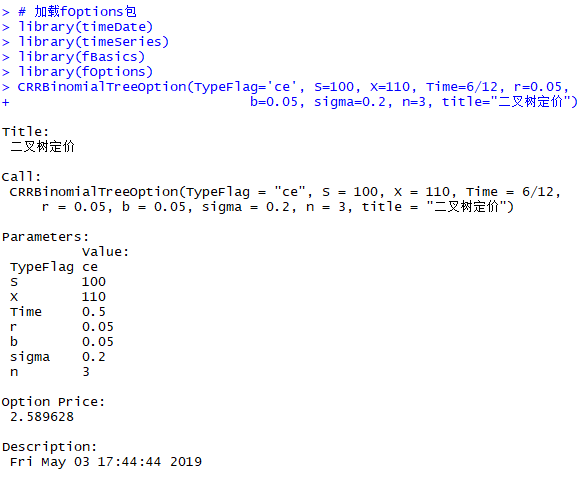
\includegraphics[height=8cm]{Rerchashu.png}
		\bicaption{使用R进行二叉树定价}{Binomial tree pricing by using R}
		\label{fig:xfig1}
	\end{figure}
	
	在上图中,可以知道二叉树定价的价格是2.589628。
	
	在R的fOptions这个包中,有一个GBSOption函数可以间接的求出Black-Schools模型的定价结果,下面给出BS模型的定价结果,用来做比较。(这里令S=100,X=110,Time=0.5,r=0.05,b=0.05,sigma=0.2)具体结果如下图所示:
	
	\begin{figure}[htb] % use float package if you want it here
		\centering
		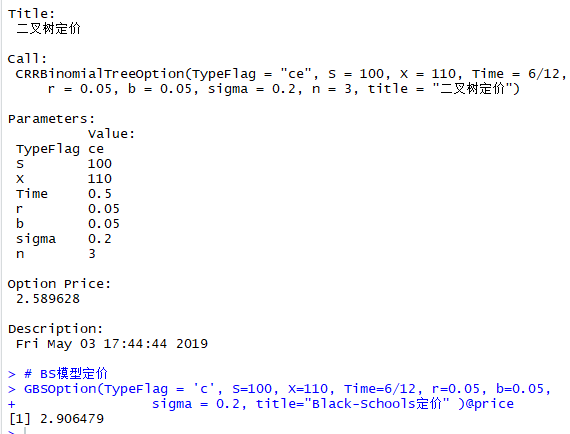
\includegraphics[height=5cm]{BSR.png}
		\bicaption{BS模型验证二叉树模型结果}{ }
		\label{fig:xfig1}
	\end{figure}

	从上述的结果中个,可以知道二叉树定价的价格为2.589628,但是Black-Schools期权定价模型的价格为2.906479,两者价格相差不大。
	下面的例子开始绘制二叉树定价的树状图。由于二叉树定价的过程不太好表述,所以可以绘制一张图来清晰的表达二叉树的结果。具体的图像如下所示:
	
	\begin{figure}[htb] % use float package if you want it here
		\centering
		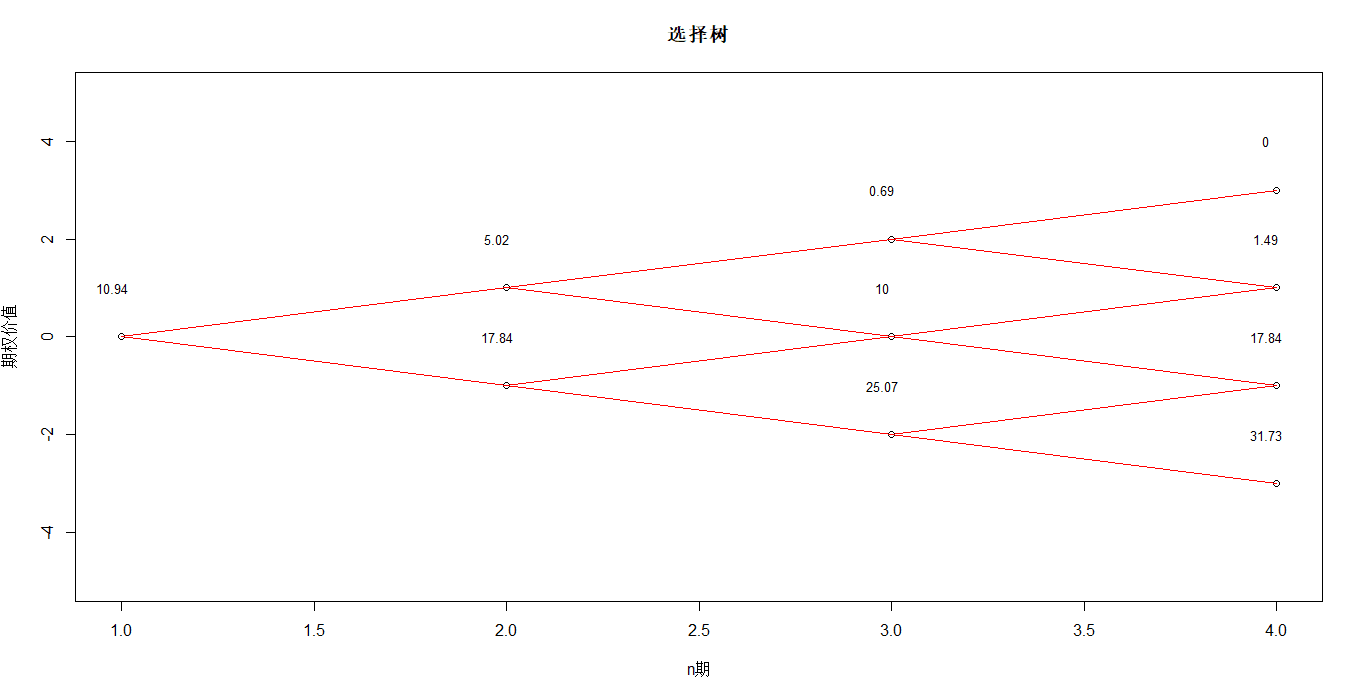
\includegraphics[height=5cm]{Rhuizhi1.png}
		\bicaption{R实现二叉树定价模型的结果绘制}{ }
		\label{fig:xfig1}
	\end{figure}

	从上图,可以清晰地看出二叉树期权定价的结果。

	当然,R也能绘制出20期期权定价的结果:
	
	\begin{figure}[htb] % use float package if you want it here
		\centering
		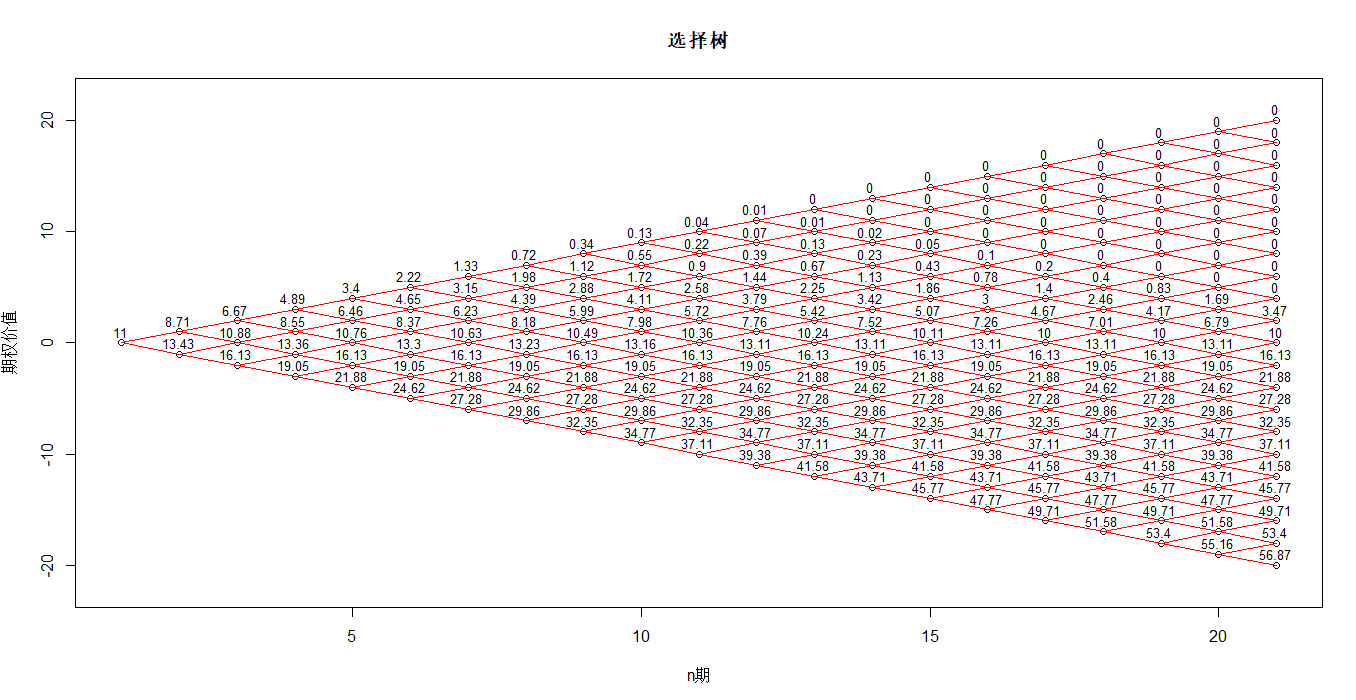
\includegraphics[height=7cm]{R20tu.png}
		\bicaption{20期期权定价结果图}{ }
		\label{fig:xfig1}
	\end{figure}
	
	
	\begin{figure}[htb] % use float package if you want it here
		\centering
		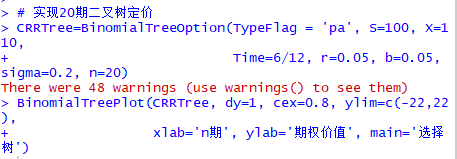
\includegraphics[height=5cm]{R20code.png}
		\bicaption{绘制20期期权定价代码}{ }
		\label{fig:xfig1}
	\end{figure}




\subsection{SAS实现二叉树定价模型}
	当然,SAS语言也可以像R语言一样,有着自己的二叉树期权定价函数。但是,也可以用SAS程序进行10期期权的二叉树定价,具体的实现过程如下各图:
	
	在下图中,可以知道:第0期股价S$_{0}$为100,$u=1.1,d=0.9$,各期无风险利率为$ r_{f}=0.05 $,期权的执行价格为$X=100$。
	
	首先输出的是SAS语言进行二叉树定价实现图。图中左边显示的是SAS的资源管理器和结果,中间显示的是日志窗口,最右边显示的是增强型编辑器窗口。
	
	\begin{figure}[htb] % use float package if you want it here
		\centering
		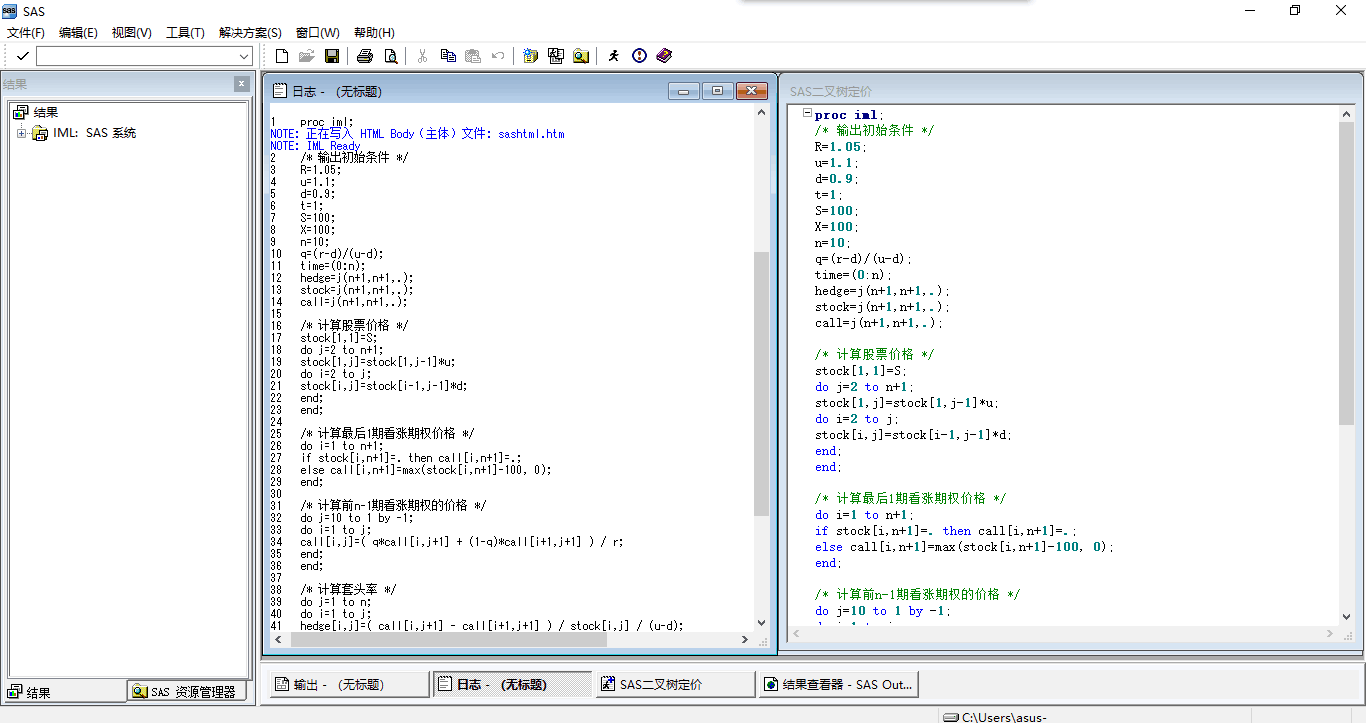
\includegraphics[height=5cm]{SASerchashu1.png}
		\bicaption{SAS语言进行二叉树定价实现}{ }
		\label{fig:xfig1}
	\end{figure}
	
	接下来输出的是10期模型各期期末股票价格变动图。
	
	\begin{figure}[htb] % use float package if you want it here
		\centering
		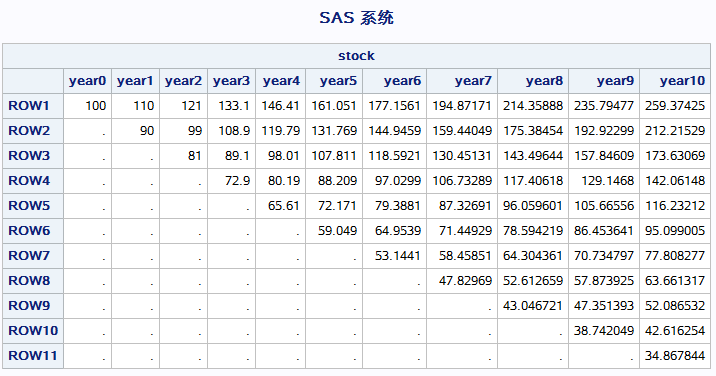
\includegraphics[height=5cm]{SASerchashu2.png}
		\bicaption{10期二叉树模型各期期末股票价格变动图}{ }
		\label{fig:xfig1}
	\end{figure}
	
	接下来输出的是10期模型各期期末的期权价格计算图。
	
	\begin{figure}[htb] % use float package if you want it here
		\centering
		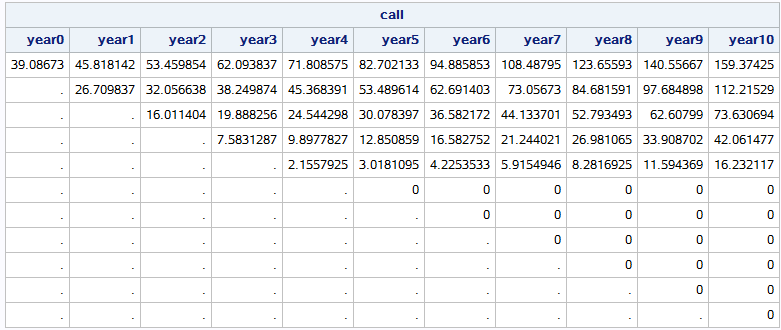
\includegraphics[height=5cm]{SASerchashu3.png}
		\bicaption{10期二叉树模型各期期末期权价格变动图}{ }
		\label{fig:xfig1}
	\end{figure}
	
	接下来输出的是:
	
	\begin{figure}[htb] % use float package if you want it here
		\centering
		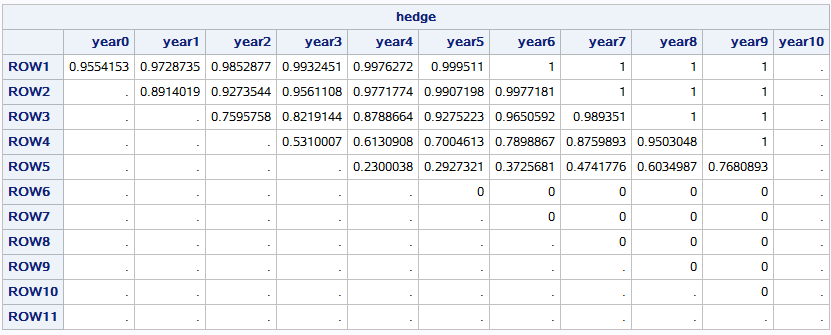
\includegraphics[height=5cm]{SASerchashu4.png}
		\bicaption{10期二叉树模型 }{ }
		\label{fig:xfig1}
	\end{figure}
	
%%	强制换页
\clearpage	

\subsection{Python实现二叉树模型的准备工作}
	二叉树期权定价模型中,标的资产价格在每一时间节点都有上升和下降的两种可能性。由于期权是标的资产的衍生工具,因此二叉树期权定价模型基于离散时间跟踪标的资产,它可以为欧式期权、美式期权,以及百慕大期权定价。
	
\subsubsection{编写StockOption类}
	利用Python运行多种期权定价方法前,先编写一个StockOption类,相当于SAS的封装宏一样,存储好股票期权的通用计算方法。将代码存为StockOption.py文件放在当前的工作目录,等待调用即可。即下图所示:
	
	\begin{figure}[htb] % use float package if you want it here
		\centering
		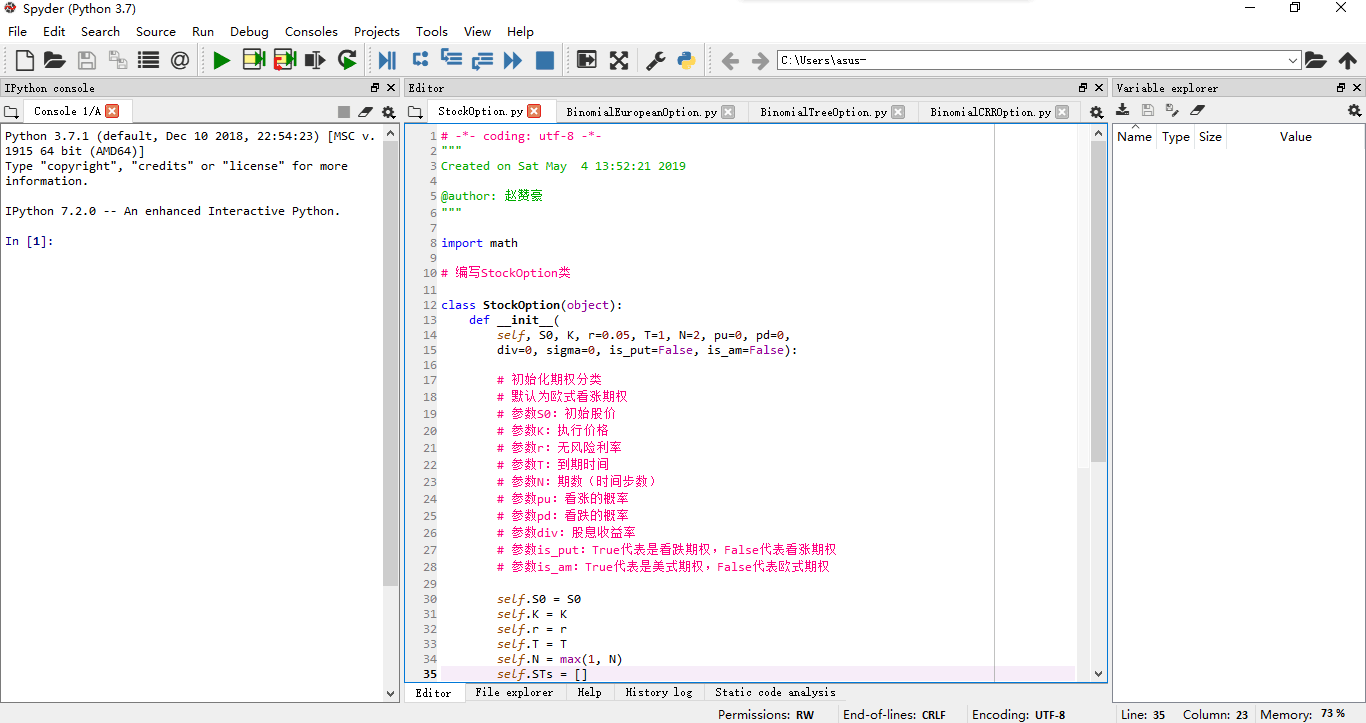
\includegraphics[height=5cm]{StockOption.png}
		\bicaption{StockOption类的编写 }{ }
		\label{fig:xfig1}
	\end{figure}

	标的资产的当前价格、行权价格、无风险利率、到期时间和时间步长的取值是期权定价所需的通用属性。其中,params变量是一个字典对象,接受模型所需的附加信息。时间步长dt和贴现率df在运行定价程序时可以反复使用。
	
\subsubsection{编写BinomialEuropeanOption类}
	Python包含对欧式期权进行二叉树定价的BinomialEuropeanOption类,该类与StockOption类使用同一期权通用属性。
	
	BinomialEuropeanOption类的定价方法是解决此类问题的通用方法。该方法调用\_setup\_parameters\_建立所需的模型参数,再调用\_initialize\_stock\_price\_tree预测T期的股票价格。最后调用私有的方法\_\_begin\_tree\_traversal\_\_,初始化收益值数组并存储折现收益值,该方法将遍历二叉树至当前结点。收益树节点作为NumPy数组对象返回,其中欧式期权的当前价值出现在初始节点。
	
	\begin{figure}[htb] % use float package if you want it here
		\centering
		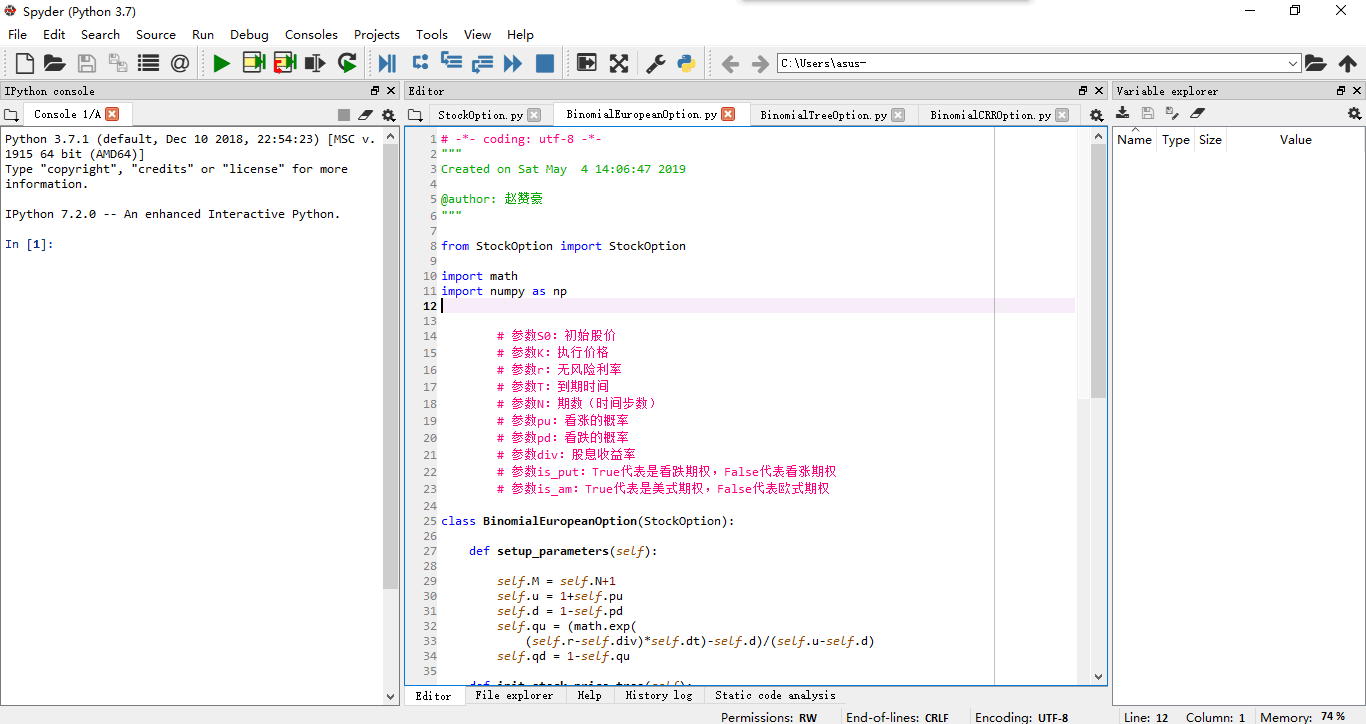
\includegraphics[height=5cm]{BinomialEuropeanOption.png}
		\bicaption{BinomialEuropeanOption类的编写 }{ }
		\label{fig:xfig1}
	\end{figure}

	需要注意的是,以双下划线开头的方法叫做私有方法,只能在同一类中访问。以单下划线开头的方法是受保护的方法,该方法可能被子类覆盖。不以下划线开头的方法为公共函数,可以从任何对象中使用。因为我曾经看过一段时间的Java,这和Java有些相似。
	
\subsubsection{编写BinomialTreeOption类}
	编写BinomialTreeOption类的主要目的是为了给美式期权定价。与欧式期权不同,美式期权可以在到期日前任意时间行权。用Python实现美式期权定价时,需要创建一个名为BinomialTreeOption的类。
	
	\begin{figure}[htb] % use float package if you want it here
		\centering
		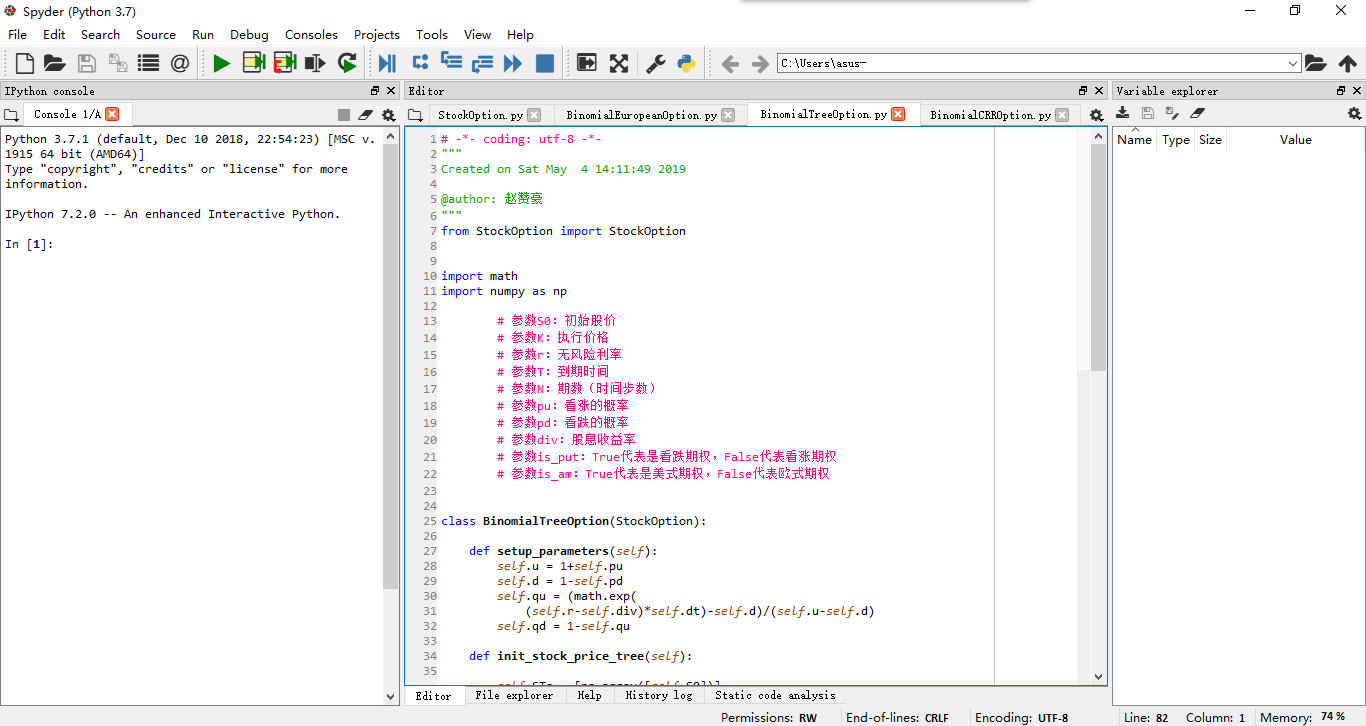
\includegraphics[height=5cm]{BinomialTreeOption.png}
		\bicaption{BinomialTreeOption类的编写 }{ }
		\label{fig:xfig1}
	\end{figure}

\subsubsection{编写BinomialCRROption类}
	创建一个BinomialCRROption类,可以为欧式期权和美式期权同时定价。
	
	\begin{figure}[htb] % use float package if you want it here
		\centering
		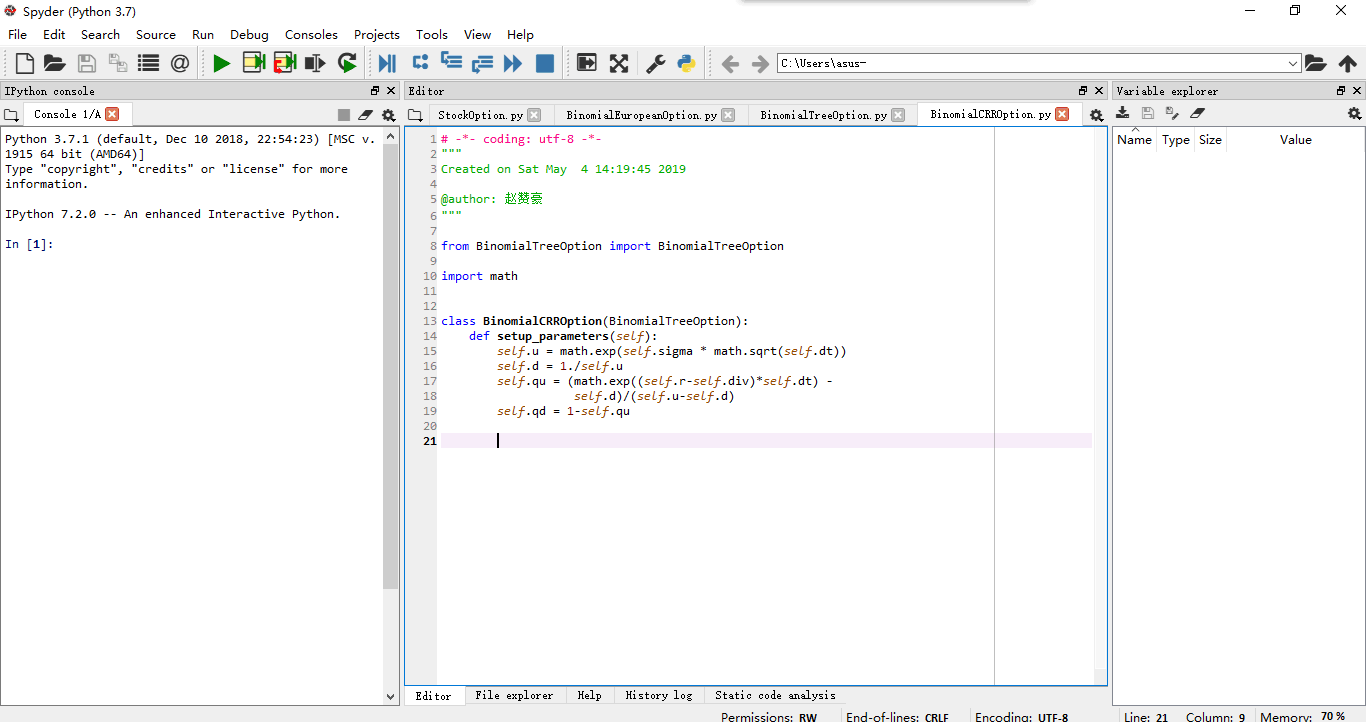
\includegraphics[height=5cm]{BinomialCRROption.png}
		\bicaption{BinomialCRROption类的编写 }{ }
		\label{fig:xfig1}
	\end{figure}



\subsection{Python实现二叉树定价模型}
	首先,我个人安装的是Python3.7.1+Anaconda3,在Anaconda3的集成环境中,有一个加Spyder的IDE。打开Spyder,然后打开工作目录下的StockOption.py,BinomialEuropeanOption.py,BinomialTreeOption.py,BinomialCRROption.py这四个.py文件。
	
	然后,依次运行StockOption.py,BinomialEuropeanOption.py,BinomialTreeOption.py,BinomialCRROption.py(按住F5即可运行)。运行结果如下图所示:
	
	\begin{figure}[htb] % use float package if you want it here
		\centering
		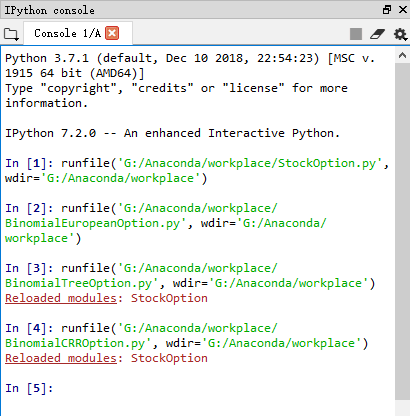
\includegraphics[height=5cm]{python1.png}
		\bicaption{Python依次运行编辑好的类文件}{ }
		\label{fig:xfig1}
	\end{figure}
	
	接下来,选用不同的类给期权进行定价。
	
	首先,给欧式看跌期权进行定价。假设在欧式看跌期权中,初始股价为50元,执行价格是52元,无风险利率是0.05,到期时间是2年,期数是2期,看涨的概率是0.2,看跌的概率是0.2。

	然后,给美式看跌期权定价。假设在美式看跌期权中,初始股价为50元,执行价格是52元,无风险利率是0.05,到期时间是2年,期数是2期,看涨的概率是0.2,看跌的概率是0.2。
	
	二叉树模型下的欧式看涨期权和美式看涨期权,得到的结果如下图:
	
	从下图中,可知,使用二叉树期权定价模型,得出欧式看跌期权的期权现值为4.1926542806038585元,得出美式看跌期权的期权现值为5.089632474198373元。
	\begin{figure}
		\begin{minipage}{0.48\textwidth}
			\centering
			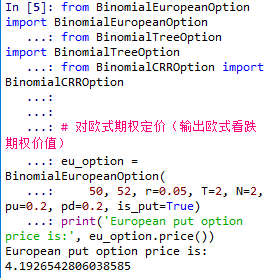
\includegraphics[height=5cm]{euoption.png}
			\caption{欧式看跌期权}
			\label{fig:parallel1}
		\end{minipage}\hfill
		\begin{minipage}{0.48\textwidth}
			\centering
			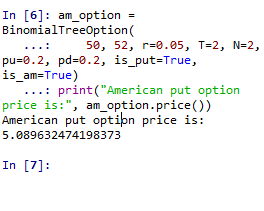
\includegraphics[height=5cm]{amoption.png}
			\caption{美式看跌期权}
			\label{fig:parallel2}
		\end{minipage}
	\end{figure}

	为什么同等条件下的欧式看跌期权和美式看跌期权的期权现值,美式看跌期权更高呢?因为美式期权可以在到期日前任意一天时点行权,欧式期权只能在到期日行权,因此美式期权的灵活性使得其价值不会低于对等的欧式期权的价值。
	
	若美式看涨期权的标的资产为不支付股息的股票,其对欧式看涨期权可能没有额外的价值。根据货币的时间价值理论,期权到期前行权比以相同行权价格在未来某个时间行权收益更小。对于不分配股息的实值美式看涨期权,期权持有人没有提前行权的动机。

	紧接着,使用CRR模型为欧式期权和美式期权进行定价。
	
	\begin{figure}[htb] % use float package if you want it here
		\centering
		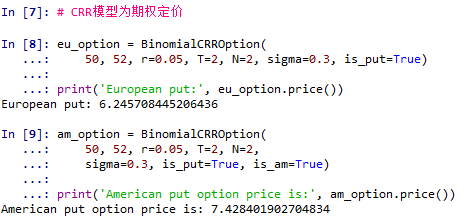
\includegraphics[height=5cm]{python2.png}
		\bicaption{CRR模型给期权定价}{ }
		\label{fig:xfig1}
	\end{figure}



%%%%%%%%%%%%%%%%% Black-Schools定价模型

\section{Black-Schools期权定价模型实现}

\subsection{R实现BS期权定价模型}
	在R中有个GBSOption函数可以间接的求出Black-Schools模型的定价结果。
	具体结果请看上述。
	
\subsection{SAS实现BS期权定价模型}
	SAS实现BS期权定价模型:
	
	\begin{figure}[htb] % use float package if you want it here
		\centering
		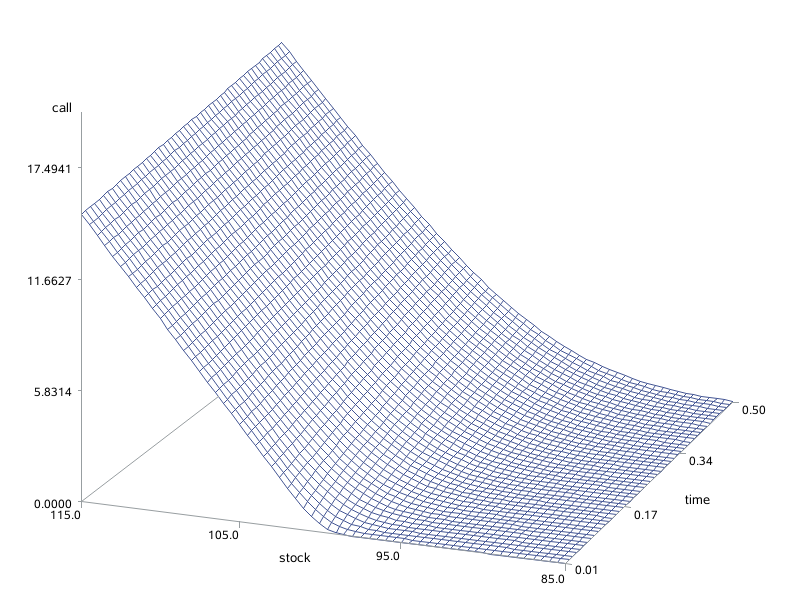
\includegraphics[height=5cm]{calloptionsas.png}
		\bicaption{欧式看涨期权价值的变动 }{ }
		\label{fig:xfig1}
	\end{figure}


	
	\begin{figure}[htb] % use float package if you want it here
		\centering
		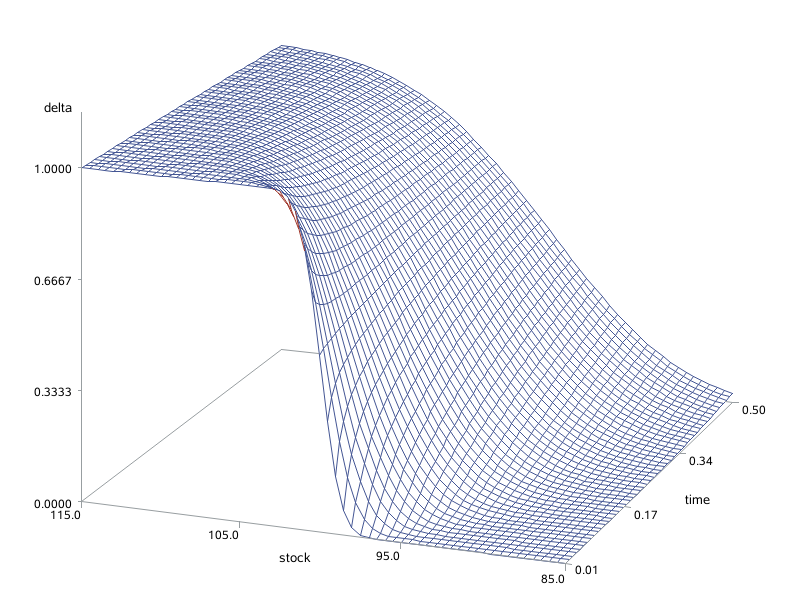
\includegraphics[height=5cm]{deltasas.png}
		\bicaption{欧式看涨期权的delta值随到期时间T、执行价格K的变化(SAS)}{ }
		\label{fig:xfig1}
	\end{figure}
	
	
	\begin{figure}[htb] % use float package if you want it here
		\centering
		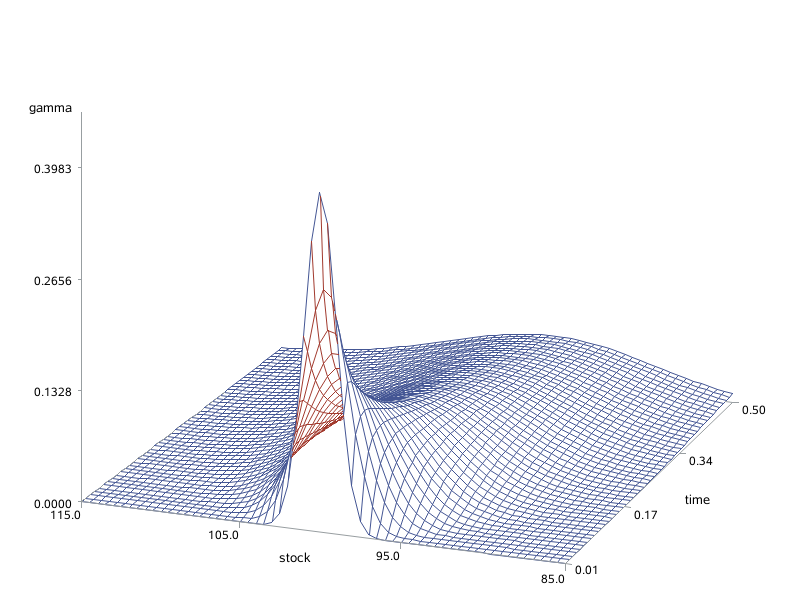
\includegraphics[height=5cm]{gammasas.png}
		\bicaption{欧式看涨期权的gamma值随到期时间T、执行价格K的变化}{ }
		\label{fig:xfig1}
	\end{figure}
	
		
	
	\begin{figure}[htb] % use float package if you want it here
		\centering
		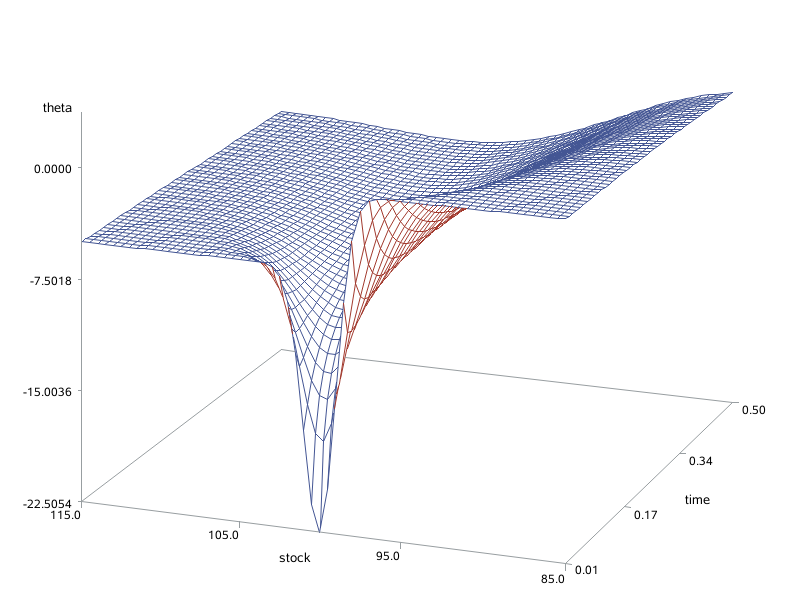
\includegraphics[height=5cm]{thetasas.png}
		\bicaption{欧式看涨期权的theta值随到期时间T、执行价格K的变化}{ }
		\label{fig:xfig1}
	\end{figure}
	
	
	
	
	
	\begin{figure}[htb] % use float package if you want it here
		\centering
		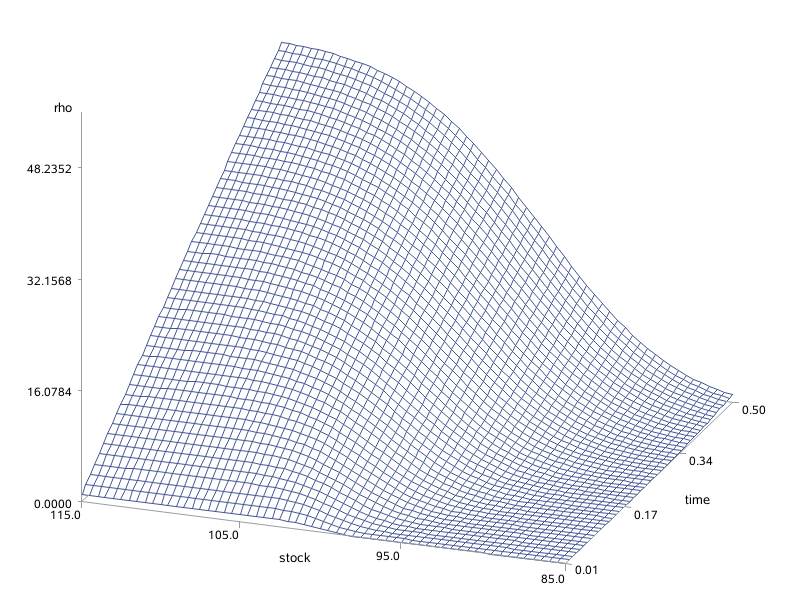
\includegraphics[height=5cm]{rhosas.png}
		\bicaption{欧式看涨期权的rho值随到期时间T、执行价格K的变化}{ }
		\label{fig:xfig1}
	\end{figure}
	
	
	
	
	\begin{figure}[htb] % use float package if you want it here
		\centering
		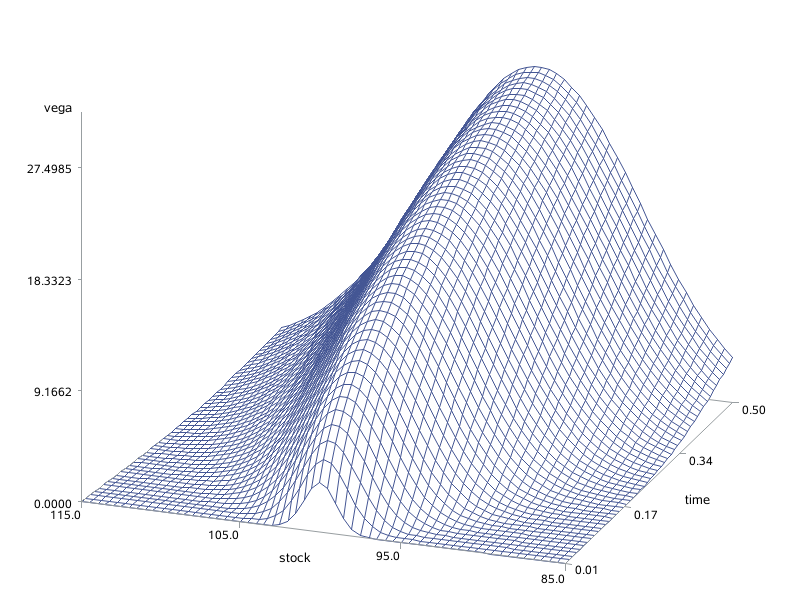
\includegraphics[height=5cm]{vegasas.png}
		\bicaption{欧式看涨期权的vega值随到期时间T、执行价格K的变化}{ }
		\label{fig:xfig1}
	\end{figure}
	
	
	
	
	
%%	强制换页
\clearpage		
\subsection{Python实现BS期权定价模型}
	自从Black,Scholes和Merton(BSM)在1973年发表了重要的论文后,BSM模型(连续市场模型)及相关的期权定价公式就被认为是期权定价的基准。其原因是,他们在一个简单但又具有一定现实意义的设定下提供了封闭解。两篇论文中推出的原始公式建立在两种不同的观点上。Black和Scholes提出的论点是均衡论点,他们认为一个无风险的资产组合在均衡收益,应该为无风险利率。Merton的论点则更为广泛地被应用,该论点认为(欧式)期权的价值应该等于能够完全复制该期权截止日期的收益,且具有适宜的交易策略的资产组合价值。

	几年后,Cox,Ross和Rubinstein(CRR)在1979年提出了二项式期权定价模型。该模型假定一个在离散时间和离散状态空间上的BSM经济体。BSM模型需要比较高深的数学,而且还需要求解偏微分方程,不过CRR分析只需要基本的概率论知识。直到今天,当很多人想用简单、直观的方法来讨论期权时,CRR用来代表不确定性的二叉树仍是重要的工具。而且,他们的数值方法不仅可以用于欧式期权定价,也可以很容易地用于美式期权定价。
	
	这两个市场模型的主要特征都是完全性:每个在未来时点到期的未定权益,都可以用两种可交易的资产——一个风险资产(比如指数或股票)和一个无风险债券的交易策略来复制。此外,当连续两期之间的时间间隔趋近于0时,CRR模型就会收敛为BSM模型。从这个角度来看,两个模型是一致的。

\subsubsection{Black-Scholes-Merton模型}
	在接下来的部分,我们主要研究欧式期权。所以,没有特别的说明,本节的“期权”就是欧式期权。为了更好地认识到期权价值对模型和期权参数的依赖情况,选取如下参数的期权作为案例来进行分析。
	
	\begin{enumerate}
		\item S$_{0}$=100:初始水平
		\item K=100:执行价格
		\item T=1.0:到期时间(年)
		\item r=0.05:无风险短期利率
		\item $\sigma$=0.2:指数的波动率
		\item t=0:定价日,即当期
	\end{enumerate}
	
	利用Python实现欧式看涨期权和看跌期权的定价公式,同时还包含了以上参数及看涨期权的图形输出,绘制的图形如下所示。以上参数和看跌期权的图形输出。每一个子图都只是改变一个基本参数得到的结果。
	
	
	
	\begin{figure}[htb] % use float package if you want it here
		\centering
		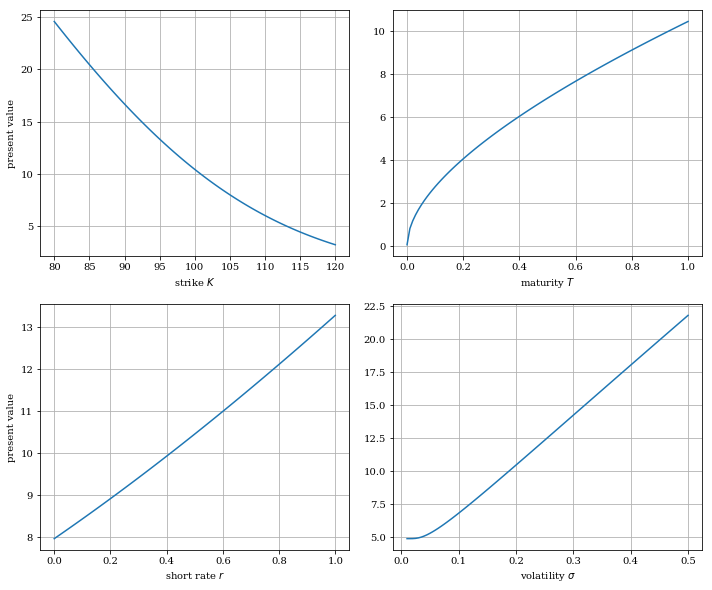
\includegraphics[height=5cm]{calloptionBS.png}
		\bicaption{欧式看涨期权价值随执行价格K、到期时间T、短期利率r、波动率$\sigma$的变动 }{ }
		\label{fig:xfig1}
	\end{figure}
	
	\begin{figure}[htb] % use float package if you want it here
		\centering
		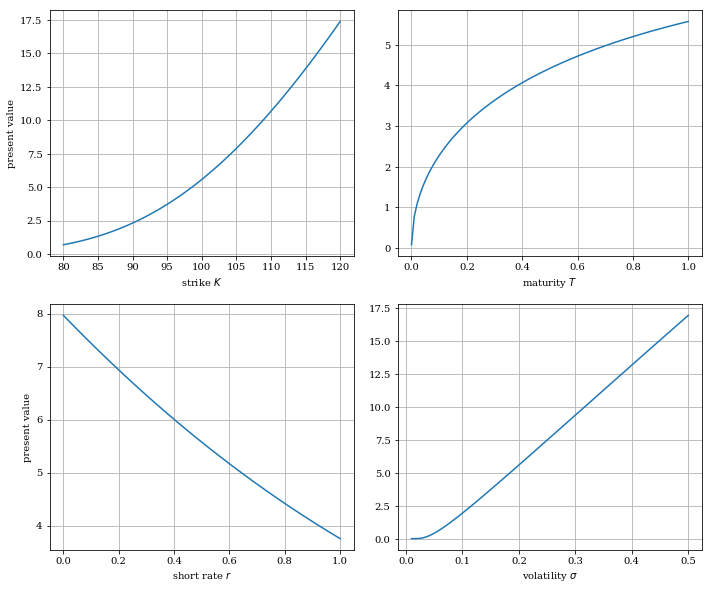
\includegraphics[height=5cm]{putoptionBS.png}
		\bicaption{欧式看跌期权价值随执行价格K、到期时间T、短期利率r、波动率$\sigma$的变动 }{ }
		\label{fig:xfig1}
	\end{figure}
	
	首先,价值状况进行比较。平价看涨期权($K=S_{0}=100,ATM$)的价值为10.4,远高于只值5.6的看跌期权,期权价内的程度越高(看涨期权:K<100;看跌期权:K>100,ITM),其价值也就越高。当期权价外的程度越高(看涨期权:K100;看跌期权:K<100,OTM),价值则越低。
	
	然后看到期时间,到期时间越长,期权的价值就越高。不过有的欧式期权并不是这样的,比如说深位价内欧式看涨期权。
	
	然后再看短期利率,短期利率的上升会增加看涨期权的价值,但是同时也会降低看跌期权的价值。在风险中性的条件下,指数随着短期利率的变动,而短期利率上涨越高对看涨期权就越有利,对看跌期权就越不利。
	
	最后看波动率,较高的波动率同时提高了看涨期权和看跌期权的价值,原因是两者在到期日变成价内的可能性都增加了。
	
	
	
	
	
	
	
\subsubsection{Black-Scholes-Merton模型的Greeks}
	
	
	
	\begin{figure}[htb] % use float package if you want it here
		\centering
		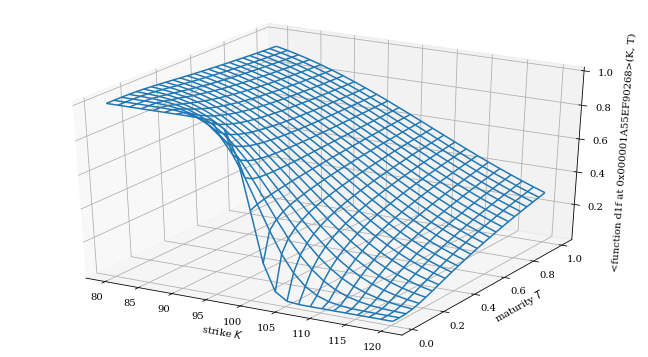
\includegraphics[height=5cm]{deltapy.png}
		\bicaption{欧式看涨期权的delta值随到期时间T、执行价格K的变化}{ }
		\label{fig:xfig1}
	\end{figure}
	
	
	
	
	
	\begin{figure}[htb] % use float package if you want it here
		\centering
		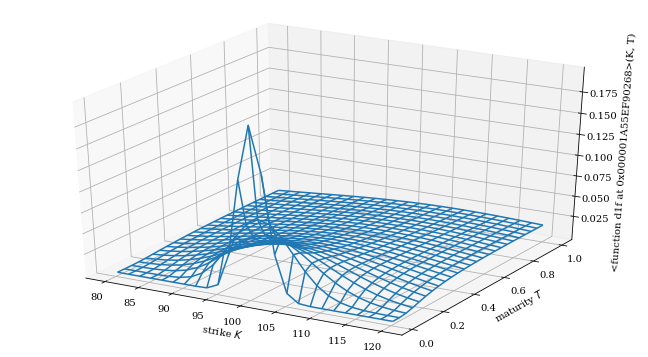
\includegraphics[height=5cm]{gammapy.png}
		\bicaption{欧式看涨期权的gamma值随到期时间T、执行价格K的变化}{ }
		\label{fig:xfig1}
	\end{figure}
	


	
	
	
	\begin{figure}[htb] % use float package if you want it here
		\centering
		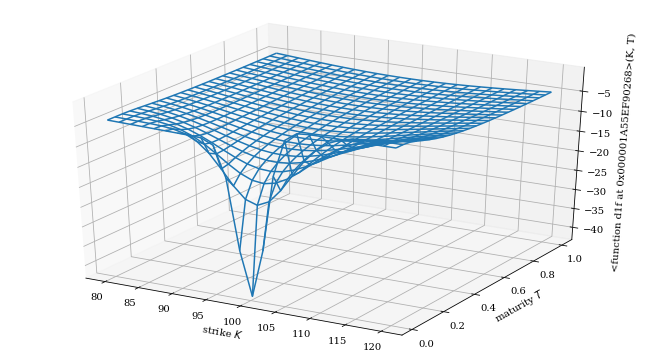
\includegraphics[height=5cm]{thetapy.png}
		\bicaption{欧式看涨期权的theta值随到期时间T、执行价格K的变化}{ }
		\label{fig:xfig1}
	\end{figure}





	\begin{figure}[htb] % use float package if you want it here
		\centering
		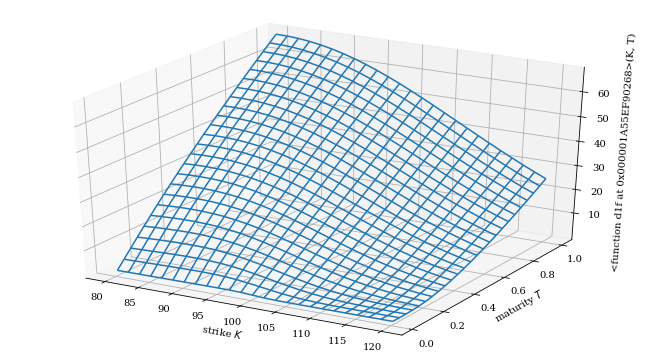
\includegraphics[height=5cm]{rhopy.png}
		\bicaption{欧式看涨期权的rho值随到期时间T、执行价格K的变化}{ }
		\label{fig:xfig1}
	\end{figure}




	\begin{figure}[htb] % use float package if you want it here
		\centering
		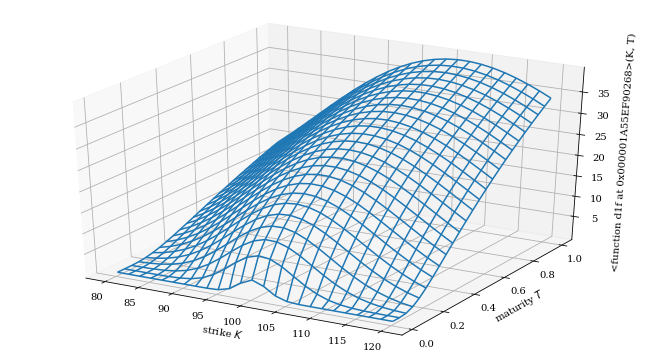
\includegraphics[height=5cm]{vegapy.png}
		\bicaption{欧式看涨期权的vega值随到期时间T、执行价格K的变化}{ }
		\label{fig:xfig1}
	\end{figure}
	
	
	
\section{蒙特卡罗期权定价模型实现}

\subsection{R实现蒙特卡罗期权定价模型}

\subsection{SAS实现蒙特卡罗期权定价模型}

\subsection{Python实现蒙特卡罗期权定价模型}








